\section{Grundlagen der Datenanalyse}

Mathematisch ausgedrückt besteht eine Zeitreihe (im englischen auch \enquote{time series} genannt) aus einer endlichen Menge an zeitlich aufsteigend sortierten Messwerten $x_{t_1},x_{t_2},...,x_{t_T};  x_{t_k} \in \mathbb{R}^n, k=1,2,...,T$, wofür $t_1 < t_2 < t_T $ gilt.\footcite[Vgl.][1]{Deistler.2018b} Zeitreihendaten sind in verschiedenen Feldern zu finden, beispielsweise im Bereich der Aktienmärkte, wo die Preise der einzelnen Kurse abgebildet werden, im Bereich der Gesundheitsforschung, wo die Ansteckungsrate ansteckender Krankheiten wie Covid-19 verfolgt wird oder im Bereich der Sozialwissenschaften, in welchen der Verlauf von Geburtsraten über die Zeit analysiert werden soll.\footcite[Vgl.][1]{Shumway.2017b} In \autoref{abb:BeispielZeitreihe} findet sich beispielhaft die Zeitreihe der verimpften Dosen des COVID-19 Impfstoffes im Januar 2021.

\begin{figure}[H]
\centering
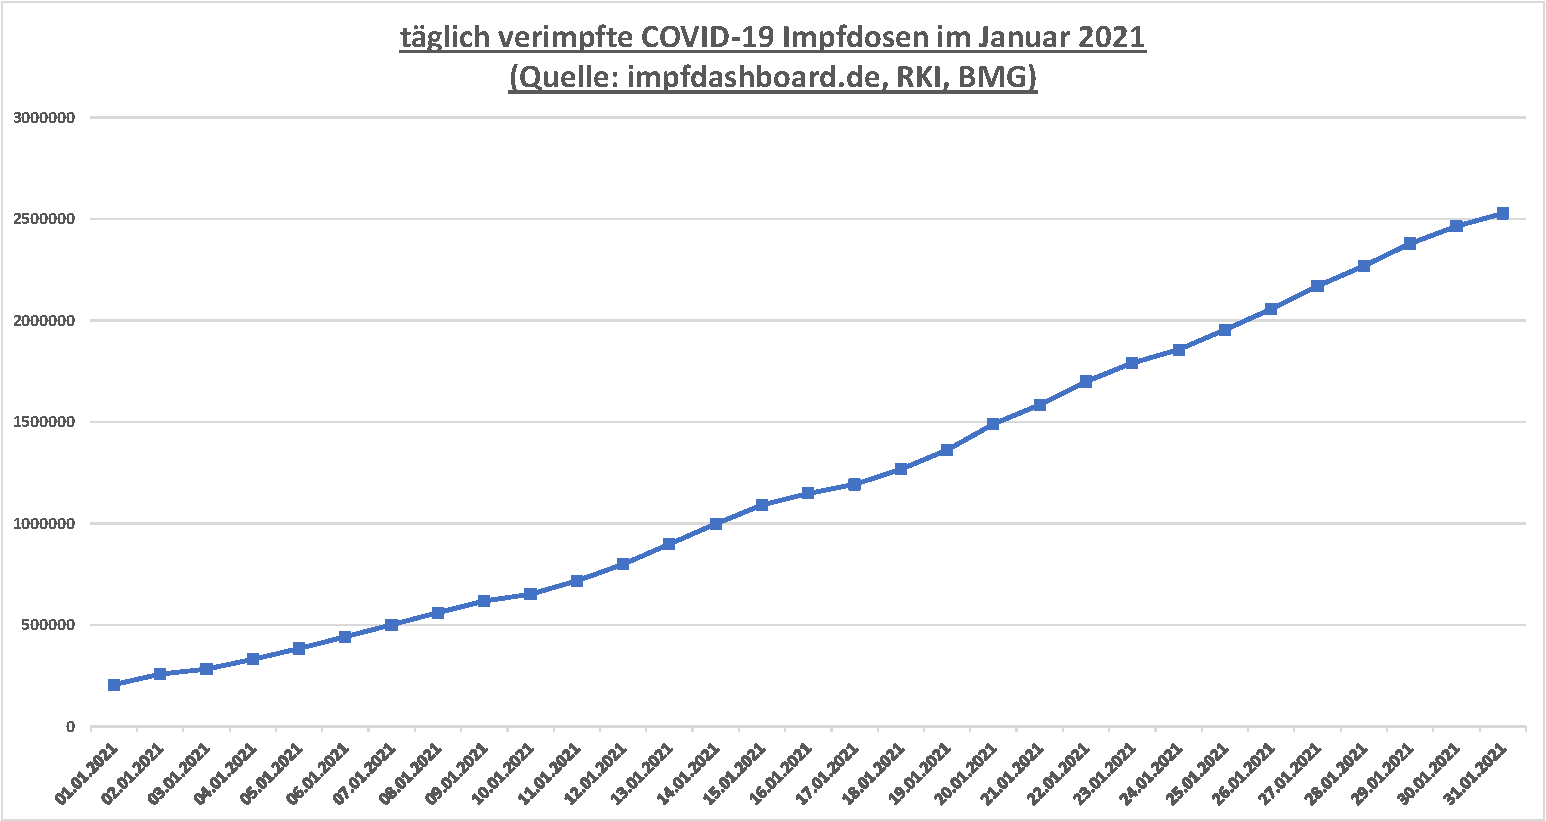
\includegraphics[width=\textwidth]{graphics/Beispiel-Zeitreihe.pdf}
\caption{Beispielhafte Zeitreihe aus dem Januar 2021}
\label{abb:BeispielZeitreihe}
\end{figure}

Die möglichen Anwendungen in der Informatik sind ebenfalls vielzählig. So können über virtuelle oder physikalische Sensoren Messwerte, wie beispielsweise die CPU Auslastung eines gegebenen Servers über die Zeit oder Temperaturmessungen eines \ac{IoT} Gerätes über die Zeit gemacht und gespeichert werden.

Ein wichtiges Merkmal von Zeitreihen ist die Distanz zwischen den Messwerten, im Sinne der Messfrequenz, in welcher Daten betrachtet werden. \Todo{belegen} Ist eine Zeitreihe äquidistant, wurde mit gleichbleibender Frequenz gemessen und die zeitliche Distanz zwischen einzelnen Messwerten ist gleich. Für die in dieser Arbeit diskutierten Auswertungsarten wird eine Äquidistanz der gemessenen Daten angenommen, da andernfalls ein Bias bei der Analyse nicht ausgeschlossen werden kann. Gleichfalls ist es technisch möglich einzelne, nicht äquidistante Messwerte auszusortieren. Die in \autoref{abb:BeispielZeitreihe} abgebildete Zeitreihe ist äquidistant, da die Werte einmal am Tag gesammelt erhoben wurden.


\Todo{Definition Zeitreihendaten}
\Todo{Definition Datenanalyse}

Bei der Verarbeitung von Daten ist zu beachten, dass der Wert, bzw. die Erkentnisse die aus den Daten abgleitet werden können, über die Zeit reduziert wird. \footcite[Vgl. auch im Folgenden][]{NucleusResarchInc..2012} In einer Analyse, die in \autoref{abb:DataHalflife} dargestellt wird, erhob Nucleus Research die Zahl, dass Daten für taktische Entscheidende nach maximal 30 Minuten die Hälfte des Wertes eingebüßt hat. Für operative Entscheidende ist die durchschnittliche Halbwertszeit nach acht Stunden erreicht, für strategische Entscheidende nach ca. 56 Stunden, also nach über 2 Tagen.
\begin{figure}[H]
\centering
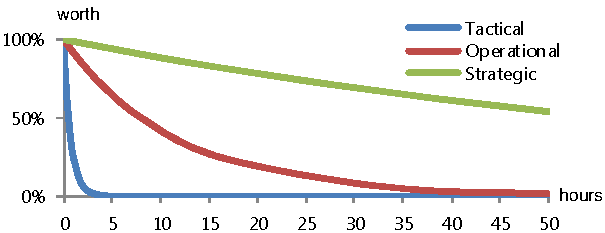
\includegraphics[width=\textwidth]{graphics/half-life-data.pdf}
\caption[Die Halbwertszeit von Daten]{Die Halbwertszeit von Daten\footnotemark}
\label{abb:DataHalflife}
\end{figure}
\footnotetext{Mit Änderungen entnommen aus: \cite{NucleusResarchInc..2012}}
Aus diesen abweichenden Halbwertszeiten und damit aus den abweichenden Zeiträumen, in denen die erhobenen Daten den höchsten Wert haben, ergibt sich die Notwendigkeit von verschiedenen Datenverarbeitungsstrategien, um entsprechend strategischen, taktischen und operativen Entscheidenden die werthaltigsten Daten als Entscheidungsgrundlage zu präsentieren.

\Todo{Kategorien der Datenentscheider}


% \Todo{Grafik Data Analytics Pipeline}
\begin{figure}[H]
\centering
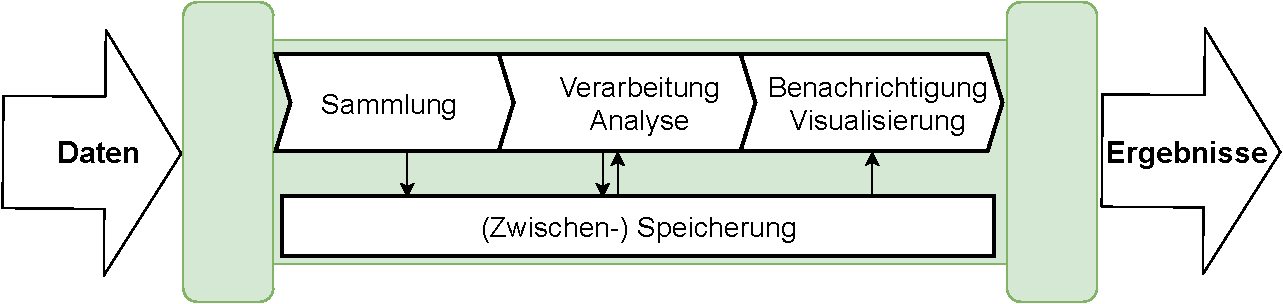
\includegraphics[width=\textwidth]{graphics/DataPipeline.pdf}
\caption{Aufbau und Ablauf in einer Data Pipeline}
\label{abb:DataPipeline}
\end{figure}
\Todo{Quellenangabe}


\subsection{Bestehende Referenzarchitekturkategorien}
Im Bereich der Streamingarchitekturen gibt es bereits etabblierte Referenzarchitekturen, welche verschiedene mögliche Aufbauarten einer Verarbeitung von Streaming/Zeitseriendaten zeigen.

% \Todo{Lambda, Kappa, OLAP elaborieren}
\begin{figure}[H]
\centering
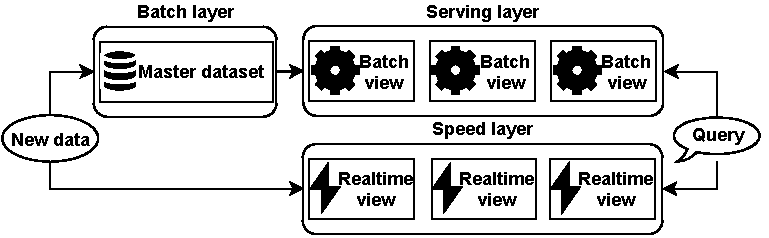
\includegraphics[width=\textwidth]{graphics/Lambda-Reference-Architecture.pdf}
\caption[$\lambda$-Datenstreaming Referenzarchitetktur]{$\lambda$-Datenstreaming Referenzarchitetktur.\footnotemark}
\label{abb:LambdaStreaming}
\end{figure}
\footnotetext{Mit Änderungen entnommen aus: \cite[][28]{Marz.2015}}
% Lambda nach \citeauthor{Marz.2015}, siehe \footcite[Vgl.][28]{Marz.2015}

Die von \citeauthor{Marz.2015} vorgestellte $\lambda$/Lambda-Architektur, welche in \autoref{abb:LambdaStreaming} gezeigt wird ist dabei eine der sehr bekannten Referenzarchitekturen. Der Name ist dabei nicht mit dem \ac{AWS} Dienst Lambda zu verwechseln, sondern ist wohl auf den gedrehten Buchstaben $\lambda$ zurückzuführen, also \reflectbox{\rotatebox[origin=c]{270}{$\lambda$}}.\footcite[Vgl. auch im Folgenden][]{Berle.27.11.2017} Die $\lambda$-Architektur sieht ausgehend von den hereingeladenen Daten zwei verschiedene Wege für die Daten vor. Zum einen den \enquote{Speed Layer}, welcher Daten direkt nach Eingang verarbeitet und nicht im Layer selbst speichert, sondern nur Aggregate oder Ergebnisse zur Verfügung stellt. Zum anderen gibt es den \enquote{Batch layer}, in welchem Daten zuerst in einem Master dataset gespeichert werden und dann in einem festen Intervall (\enquote{Batch jobs}) ausgewertet werden. Verschiedene Datenverarbeitungsintervalle machen speziell im Sinne der verschiedenen, in \autoref{abb:DataHalflife} gezeigten, Datenhalbwertszeiten Sinn. So sind manche Auswertungen, die präzise historische Daten benötigen in einem Batch layer besser möglich als in einem speed layer. Der speed layer bietet dagegen durch die Geschwindigkeit der Auswertungen die möglichkeit, agil auf erkannte Ereignisse oder Veränderungen im generellen zu reagieren.


\begin{figure}[H]
\centering
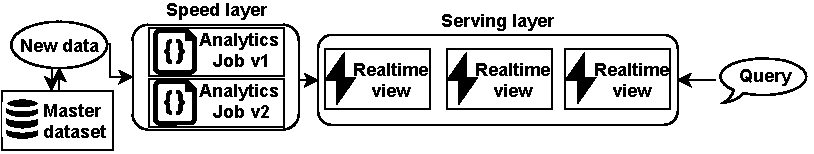
\includegraphics[width=\textwidth]{graphics/Kappa-Reference-Architecture.pdf}
\caption[$\kappa$-Datenstreaming Referenzarchitetktur]{$\kappa$-Datenstreaming Referenzarchitetktur.\footnotemark}
\label{abb:KappaStreaming}
\end{figure}
\footnotetext{Mit Änderungen entnommen aus: \cite{Kreps.2014}, \cite{Berle.27.11.2017}}

Die $\kappa$/Kappa Referenzarchitektur von \citeauthor{Kreps.2014}, dargestellt in \autoref{abb:KappaStreaming} basiert auf der $\lambda$-Architektur, spart jedoch den \enquote{Batch layer} mit zugehörigen \enquote{Batch jobs} aus. Das Konzept von Master Data existiert dabei weiterhin, jedoch in Form von Nachrichten, die in einem Messagebroker gespeichert werden. Analysen werden in Form von einzelnen, unveränderlichen Jobs über die vorhandenen Nachrichten erstellt. Wird die Analyse in irgendeiner Weise verändert (z.B. durtch Codeanpassungen) werden alle zwischengespeicherten Nachrichten erneut durch eine neue, unveränderliche Version des Jobs analysiert. Diese Unveränderlichkeit hat den Vorteil, dass keine unerwünschten Seiteneffekte durch Analysen, die gegenseitig Ergebnisse überschreiben auftreten. \Todo{elaborate on original source}

% Kappa nach \citeauthor{Kreps.2014},
% siehe \footcite[Vgl.][]{Kreps.2014}



\begin{figure}[H]
\centering
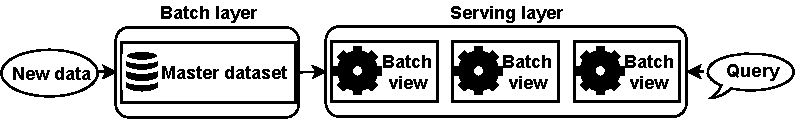
\includegraphics[width=\textwidth]{graphics/OLAP-Reference-Architecture.pdf}
\caption[OLAP Referenzarchitetktur]{OLAP Referenzarchitetktur.\footnotemark}
\label{abb:OLAPStreaming}
\end{figure}
\footnotetext{Mit Änderungen entnommen aus: \cite{Kreps.2014}}

%\ac{OLAP}
Aus der $\lambda$ Referenzarchitektur lässt sich auch eine, zur $\kappa$ Architektur gegenteilige Architektur aufzeigen, welche ein klassisches \ac{OLAP} Szenario aufzeigt. \Todo{Codd zitieren} Diese Architektur basiert, wie in \autoref{abb:OLAPStreaming} gezeigt, auf einer periodischen Verarbeitung der Daten im Master dataset. Dieses Vorgehen ist bei traditionellen Analytics weit verbreitet, bietet jedoch womöglich wichtige Einsichten erst nachdem die Datenhalbwertszeit bereits überschritten wurde.


\subsection{Arten der Auswertung}
\subsubsection{Median}
\subsubsection{Anomaliedetektion}
\subsubsection{Schwellwertüberschreitung}
\subsubsection{Trenderkennung/gleitender Durchschnitt}


\subsection{Echtzeitverarbeitung}
Gemäß der in \autoref{abb:KappaStreaming} gezeigten $\kappa$-Architektur gibt es Nutzungsfälle, in welchen eine reine Echtzeitauswertung basierend auf einer Datenquelle, wie beispielsweise dem Messagebroker Sinn machen kann. \citeauthor{Belur.2020} sieht dabei vier verschiedene Verwendungszwecke, in welchen die niedrige Verarbeitungslatenz besonders wichtig ist und den maximalen Wert aus den Daten zieht.\footcite[Vgl. auch im Folgenden][]{Belur.2020} Durch Echtzeit reporting und die Erstellung von Dashboards können aktuelle Daten schnell übersichtlich aufbereitet werden. Mittels erstellter Regeln, die Schwellwertüberschreitungen und Anomalien detektieren, können Nutzende benachrichtigt werden, sobald es zu einer Abweichung kommt. Ebenfalls sinnvoll ist Machine Learning zum auffinden von Mustern in den Daten zu verwenden, was verbesserte Anomalierkennung, Vorraussagen und ähnliche Features ermöglicht. Ein weiterer valider Usecase der $\kappa$-Architektur ist die Transformation von Daten in gewisse Zielformate, um beispielsweise Drittsysteme anzusprechen.
Requirements:
\begin{itemize}
\item Unified experience for data ingestion and edge processing
\item Versatile out-of-the-box connectivity
\item Scalable stream processing with complex transformations
\item Operationalized business rules and ML models
\item Ability to handle unstructured data and schema drift:
\item Reusability of processing logic
\item Governance and lineage
\end{itemize}

% \subsubsection{Streamanalyse}
% \begin{itemize}
% \item AWS Kinesis Data Analytics/Stream
% \item AWS Lambda
% \end{itemize}

\subsection{Datenbankseitige Verarbeitung}
\subsubsection{Datenbankabfragen}
\begin{itemize}
\item Timestream
\item Redshift
\item Athena
\item Elasticsearch
\end{itemize}

\subsubsection{Externe Analyse}
\begin{itemize}
\item Amazon EMR
\item Amazon Glue
\item AWS Lake Formation
\end{itemize}




Source -> Stream ingestion -> Stream storage -> Stream processing -> Destination

Talkingpoints gegen Streaming onprem:
Difficult to set up, Difficult to achieve high availability,
Error prone and complex to manage,
Tricky to scale, Integration requires development,Expensive to maintain

Amazon Kinesis Data Streams - Daten verfügbar in 70 Milisekunden



Amazon Kinesis Data Analytics


\subsubsection{Brokeranalyse}

\begin{itemize}
\item AWS IoT Analytics
\end{itemize}